%% STORM-PhysNet — IEEE CONFERENCE (target 6 pages)
%% documentclass: IEEEtran conference
\documentclass[conference]{IEEEtran}
\usepackage{amsmath,amssymb,amsfonts}
\usepackage{graphicx}
\usepackage{booktabs}
\usepackage{multirow}
\usepackage{cite}
\usepackage{url}
\usepackage{xcolor}
\usepackage{balance}

\title{STORM-PhysNet: Physics-Informed Multi-Horizon Forecasting of
Geostationary Relativistic Electron Flux with Transfer to Indian Longitude}

\author{
\IEEEauthorblockN{Samarth BN}
\IEEEauthorblockA{BE in Electronics and Communication\\
RV College of Engineering, Bengaluru, India\\
Email: samarthbn.ec25@rvce.edu.in}
}

\begin{document}
\maketitle

%% --------------------------------------------------------------------
\begin{abstract}
Energetic electrons above 2\,MeV at geostationary orbit (GEO) pose a
persistent internal-charging hazard for satellites. We present STORM-PhysNet,
a multi-horizon forecast model that augments a standard Transformer
encoder (temporal self-attention over the 72-hour input window) with
a learnable solar-wind propagation delay
\(\tau\) and a \(B_z\)-conditioned physics gate for simultaneous 45-minute,
6-hour, and 12-hour log-flux predictions.

On hourly GOES--OMNI data with three independent random seeds, the
\(B_z\)-gated variant (STORM-BzGate) reaches mean prediction efficiency
(PE) \(0.669\pm0.030\) at 6\,h versus \(0.648\pm0.031\) for a strong Vanilla
Transformer baseline, and improves storm-time PE from \(0.612\pm0.042\) to
\(0.674\pm0.017\). At 45\,min the Transformer exhibits high instability across
seeds (PE range: \(-0.456\) to \(+0.002\), mean \(-0.153\pm0.262\)), while STORM-BzGate
is tightly clustered near \(0.34\pm0.05\) across all seeds---a reliability
gap that is arguably more consequential operationally than the mean difference
alone. Three-seed ablations confirm
that removing the adaptive delay degrades storm PE by 3.0 percentage points;
removing the physics loss degrades it by 2.3 points. A parameter-free
ensemble of Transformer and STORM-BzGate attains PE 0.718.

Transfer to 14 months of ISRO GSAT-19 GRASP data at Indian longitude reveals
that zero-shot deployment fails (PE\(_{6h}=-2.16\)) due to sensor mismatch;
frozen-encoder fine-tuning with only \(\sim\)73K trainable parameters
(input and output projections only) recovers
PE\(_{6h}=0.564\) and achieves the best storm-time and high-flux skill of
any strategy. Learned delays fall near \(1.5\,\mathrm{h}\) on the final evaluation checkpoints, consistent with residual L1--Earth transit under typical solar-wind speeds.
\end{abstract}

\begin{IEEEkeywords}
Geostationary orbit, relativistic electrons, space weather, Transformer,
physics-informed, transfer learning, prediction efficiency, GRASP
\end{IEEEkeywords}

%% ====================================================================
\section{Introduction}
%% ====================================================================
Geostationary satellites sit inside the outer radiation belt, where
relativistic electrons (\(E>2\,\mathrm{MeV}\)) can jump by several orders of
magnitude in a few hours when a geomagnetic storm develops. Those bursts drive
internal charging and can upset or damage onboard electronics~\cite{baker2018space,horne2005wave}.
For operators of GEO assets at Indian longitudes---ISRO broadcasting,
navigation, and remote-sensing satellites among them---a forecast that is
usable at the local meridian, not only at GOES longitudes, is increasingly
useful.

Most published skill scores still come from GOES-centered data sets. When a
new instrument such as GRASP on GSAT-19 comes online, there is often only a
short calibrated record, so operators need a practical path from a data-rich
satellite to a data-scarce one without retraining everything from scratch.

Forecast models have progressed from linear filters~\cite{baker1990,perry2010}
through LSTM and hybrid deep-learning approaches~\cite{wei2018,son2022,zhang2022emd}
to recent Transformer-based architectures reporting daily-fluence PE of
0.85--0.92~\cite{sun2025fsl,tan2024tpa,sun2024swsc}. The iTransformer
of Liu et al.~\cite{liu2024itrans}, which inverts the standard attention
axis from time steps to variates, was evaluated as an alternative backbone;
the standard temporal-attention Transformer proved more consistent across
seeds and is used for all reported results. Despite these advances, two
gaps remain: (i) the short-horizon (45\,min) behavior of
Transformer architectures relative to physics-informed variants is poorly
characterized, and (ii) no systematic study has assessed transfer strategies
for Indian-longitude GEO assets such as GSAT-19.

We introduce STORM-PhysNet to address both gaps. The model couples a
standard Transformer with a learnable L1 propagation delay and a
\(B_z\)-conditioned gate, predicts 45\,min / 6\,h / 12\,h jointly, and is
evaluated under matched chronological splits and three seeds against LSTM,
MLP, CNN, and Vanilla Transformer baselines. We further report a full
GOES\(\rightarrow\)GRASP transfer suite (zero-shot, frozen, full, scratch,
few-shot) and simple interpretability checks on learned \(\tau\) and gate
activations.

%% ====================================================================
\section{Related Work}
%% ====================================================================
Camporeale~\cite{camporeale2019} summarizes common failure modes when ML is
applied to space weather (leaky splits, mismatched metrics, overstated skill).
Morley et al.~\cite{morley2018} argue for prediction efficiency against a
persistence baseline, which we adopt so that PE \(=0\) means ``no better than
holding the last value.''

On the modeling side, work moved from linear filters and empirical solar-wind
drivers~\cite{baker1990,perry2010,ling2010} to LSTM and hybrid deep
models~\cite{wei2018,son2022,zhang2022emd}, and more recently to
Transformer-style networks for GEO flux and fluence~\cite{tan2024tpa,sun2024swsc,sun2025fsl}.
Those papers mainly report daily or multi-hour skill on GOES-like targets.
Two practical gaps remain for our setting: (i) short-lead (about 45\,min)
behavior is rarely stress-tested across random seeds, and (ii) transfer from a
long GOES record to a short Indian-longitude record such as GRASP is not
benchmarked under the same splits and horizons.

Physics-informed constraints are less common in published GEO flux networks
than pure sequence models. Where they appear, they are often implemented as
loss penalties or post-hoc diagnostics rather than as an explicit delay-plus-gate
structure trained end-to-end with multi-horizon heads. Our design keeps the
Transformer backbone standard so that gains can be attributed to the delay and
gate modules rather than to a wholesale change of encoder family.

Solar-wind timing is another recurring issue. OMNI already applies a
phase-front correction from L1, yet residual timing errors of tens of minutes
are still reported~\cite{forsyth2020}. We treat that lag as a single learnable
scalar rather than a fixed offset. Cross-platform radiation-belt products
exist for other fleets~\cite{sinha2021premeve}; the specific GOES\(\rightarrow\)GRASP
path at \(\approx 82^\circ\)E, with frozen-encoder fine-tuning and few-shot
curves, is the transfer setting studied here.

\begin{figure*}[!t]
\centering
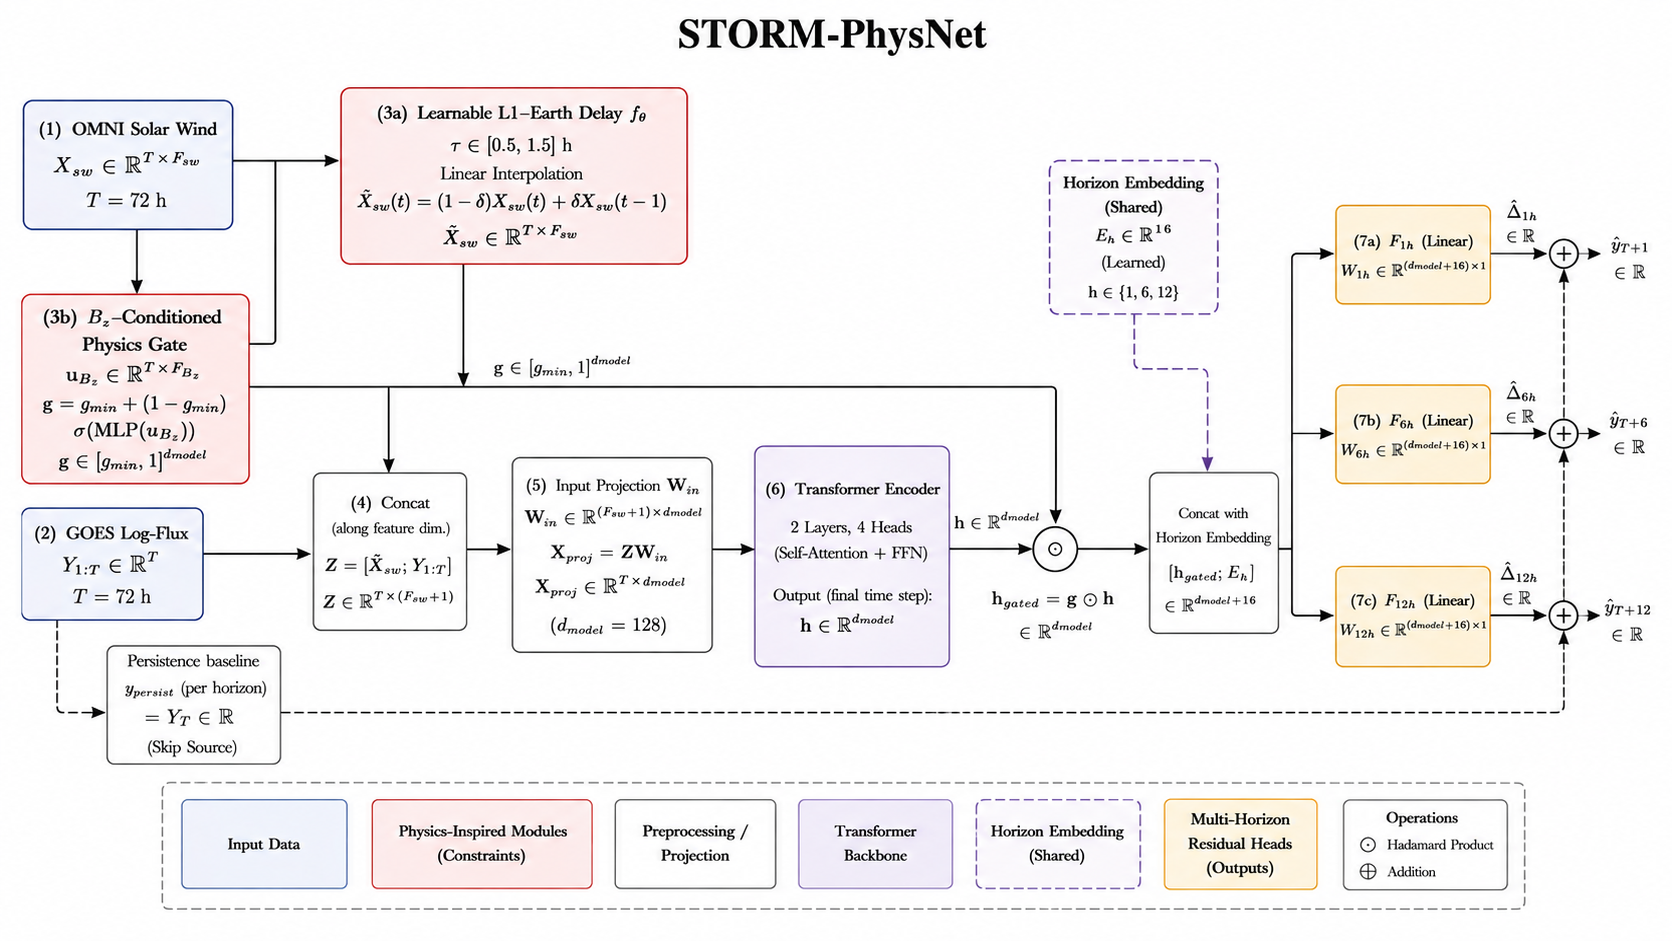
\includegraphics[width=0.95\textwidth]{figures/fig_system_architecture.png}
\caption{STORM-PhysNet: adaptive delay, temporal Transformer, \(B_z\) gate, and multi-horizon heads.}
\label{fig:arch}
\end{figure*}

\section{Data and Metrics}
%% ====================================================================
\textbf{GOES-15.} We use \(E>2\,\mathrm{MeV}\) integral electron flux from a
chronological working sample spanning approximately 2012--2016 within the
GOES-15 archive. One-minute samples are aggregated to hourly means; the
within-hour standard deviation is kept as an input feature. Flux is
\(\log_{10}\)-transformed. These measurements are merged with 16 hourly OMNI
solar-wind and geomagnetic features: solar wind speed, density, dynamic
pressure, IMF \(B_t\), \(B_z\), \(B_x\), \(B_y\), \(E_y=-V_{sw}B_z\), Dst,
Kp, AE, AL, AU, proton temperature, plasma beta, and log-flux as an
autoregressive channel. A 72\,h lookback window is used at each forecast
origin. Train/validation/test splits are chronological 70/15/15\% with no
shuffling; storms that straddle a boundary are assigned to the later split.

\textbf{GRASP} (GSAT-19, Indian longitude \(\approx82^\circ\)E) provides
14 months of GEO radiation measurements from July 2017 to September 2018 in
the declining phase of Solar Cycle 24. After alignment, GRASP supplies 15
solar-wind-related inputs versus 16 on GOES; this mismatch is the main reason
zero-shot transfer fails and motivates input-projection adaptation. Storm
windows on GRASP are defined by Dst \(\le -50\,\mathrm{nT}\) (118/1781 test
hours, 6.6\%).

\textbf{Skill score.} We use prediction efficiency~\cite{morley2018}:
\begin{equation}
\mathrm{PE}=1-\frac{\mathrm{MSE}(\hat{y},y)}{\mathrm{MSE}(y^{\mathrm{pers}},y)},
\end{equation}
reported for the full test set (PE\(_\mathrm{all}\)), storm windows
(PE\(_\mathrm{storm}\)), and the top 10\% flux samples (PE\(_\mathrm{hi}\)).
All \(\pm\) values are sample standard deviations over three seeds.
PE \(< 0\) means the model is worse than persistence.

%% ====================================================================
\section{STORM-PhysNet Architecture}
%% ====================================================================




\subsection{Adaptive Propagation Delay}
Solar wind measured at L1 reaches the magnetopause after a transit of
0.8--1.2\,h depending on speed~\cite{forsyth2020}. A learnable scalar
\(\tau\) (initialized at 1.0\,h) applies a differentiable linear interpolation
to the solar-wind channels:
\begin{equation}
\tilde{X}_{\mathrm{sw}}(t) =
(1-\alpha)\,X_{\mathrm{sw}}(t) +
\alpha\,X_{\mathrm{sw}}(t-1),
\quad\alpha=\tau-\lfloor\tau\rfloor.
\end{equation}
This allows the optimizer to recover the effective L1-to-Earth transit time
without requiring explicit spacecraft-position geometry. Across three seeds,
converged \(\tau\) concentrates near \(1.5\,\mathrm{h}\) on final checkpoints (Fig.~\ref{fig:delay}).

\subsection{\(B_z\)-Conditioned Physics Gate}
Sustained southward IMF \(B_z\) triggers dayside reconnection and ring-current
injection~\cite{horne2005wave}. A lightweight gate:
\begin{equation}
g = \sigma(w_1 B_z + w_2|B_z| + w_3 P_{\mathrm{dyn}} + b)
\end{equation}
modulates the feature representation, amplifying storm-relevant interactions
when \(B_z\) is strongly negative. Gate activations shift measurably toward
lower values during storm windows (Fig.~\ref{fig:gate}), providing
interpretable evidence that the gate tracks the physical driver.

\subsection{Transformer Backbone and Multi-Horizon Heads}
We use a standard Transformer encoder~\cite{vaswani2017} as the backbone:
each of the \(T=72\) time steps is a token; self-attention is applied
across the temporal dimension; the final time-step hidden state
\(\mathbf{h}\in\mathbb{R}^{d_{\mathrm{model}}}\) is passed to the gate and heads.
We use 3 encoder layers, \(d=128\), 4 heads, and FFN dimension 256.
Measured sizes are \(\approx3.4\times10^{5}\) parameters (STORM) versus \(\approx8.4\times10^{5}\) (Transformer).
An iTransformer variant (variate-axis attention, Liu et al.~\cite{liu2024itrans})
is implemented but not used in the reported experiments.
Three independent residual heads
project the shared latent vector to the 45\,min, 6\,h, and 12\,h forecasts,
each with a skip connection from the last-observed flux value.

\subsection{Physics Regularization Loss}
The total training objective is:
\begin{equation}
\mathcal{L} = \mathcal{L}_{\mathrm{base}} + \lambda_{\mathrm{phys}}
\sum_{t\in\mathcal{S}}\mathrm{MSE}(\hat{y}_{t+6},y_{t+6}),
\end{equation}
where \(\mathcal{S}\) is the set of storm-onset hours (\(B_z<-5\,\mathrm{nT}\),
\(P_{\mathrm{dyn}}>4\,\mathrm{nPa}\)) and \(\lambda_{\mathrm{phys}}=1.5\).
The \texttt{no\_physics} ablation sets \(\lambda_{\mathrm{phys}}=0\).

\subsection{Baselines, Training, and Ensemble}
We compare against: Vanilla Transformer (same architecture, no delay/gate),
LSTM (2 layers, 128 hidden), MLP (3 layers, 512-256-128), and CNN (3 conv
layers, kernel 5). All models share the same chronological splits. Training
uses Adam with initial learning rate \(3\times10^{-4}\), a short warmup,
cosine decay, batch size 256, and early stopping on validation
PE\(_\mathrm{all}\). STORM variants and ablations use seeds \(\{42,43,44\}\);
baselines use one seed unless stated. Transfer fine-tuning uses a lower
learning rate (\(5\times10^{-5}\)) for at most 50 epochs. The TF+BzGate
ensemble averages predictions in log-flux space at zero additional training
cost.

%% ====================================================================
\section{Results}
%% ====================================================================

\subsection{GOES Multi-Seed Performance}
Table~\ref{tab:main} and Fig.~\ref{fig:horizon} summarize
test-set results. STORM-BzGate leads on PE\(_\mathrm{all}\), PE\(_\mathrm{storm}\),
and high-flux PE at 6\,h. The gap versus the Vanilla Transformer is modest
on the full test set (\(\approx 0.02\) PE) but clearer in storm windows
(\(\approx 0.06\) PE). That pattern matches the design intent: the delay and
gate are meant to help when the driver is active, not to rewrite quiet-time
persistence.

A paired seed comparison on PE\(_\mathrm{all}\) is not significant at \(n=3\) (Cohen's \(d\approx0.40\)); we treat the bulk gain as modest and emphasize storm-time PE and short-horizon reliability.
The larger story is at 45\,min. Across the same three seeds, Transformer PE
runs from \(+0.002\) down to \(-0.456\) (mean \(-0.153\pm0.262\)). STORM-BzGate
stays between \(0.275\) and \(0.370\) (mean \(0.337\pm0.054\)). For an operator
who needs a short warning window, a model that sometimes collapses below
persistence is harder to trust than one whose PE stays in a narrow band,
even if the mean 6\,h scores look similar.

CNN performance (PE\(=0.033\)) is weak on this split. Global pooling removes
much of the phase information that moderate-activity intervals still need.
LSTM and MLP land between the CNN and the Transformer; they are useful
controls but are not the main comparison once the Transformer baseline is in
place. Averaging Transformer and STORM-BzGate outputs in log-flux space
(no extra training) reaches PE 0.718, which suggests the two models do not
fail on the same samples.

Permutation importance on the \(6\,\mathrm{h}\) head ranks \(B_z\) first, followed
by within-hour flux variability and longer solar-wind speed memory. That
ordering matches standard radiation-belt drivers and supports the choice of a
\(B_z\)-conditioned gate. Residual scatter at \(6\,\mathrm{h}\) is centered near
zero, with heavier tails on large flux jumps---the same regimes where
persistence is weakest.

\begin{table}[t]
\centering
\caption{GOES test, 6\,h PE. Multi-seed \(n=3\) for all rows. Bold: best.}
\label{tab:main}
\setlength{\tabcolsep}{3.5pt}
\begin{tabular}{lcccc}
\toprule
Model & \(n\) & PE\(_{\mathrm{all}}\) & PE\(_{\mathrm{st}}\) & PE\(_{\mathrm{hi}}\) \\
\midrule
Transformer & 3 & \(0.648\pm0.031\) & \(0.612\pm0.042\) & 0.717 \\
STORM-BzGate & 3 & \(\mathbf{0.669\pm0.030}\) & \(\mathbf{0.674\pm0.017}\) & \textbf{0.745} \\
STORM-Cathode & 3 & \(0.664\pm0.012\) & \(0.639\pm0.037\) & 0.710 \\
STORM-Cath.+Spec & 3 & \(0.666\pm0.020\) & \(0.655\pm0.021\) & 0.732 \\
STORM-Radio. & 3 & \(0.656\pm0.002\) & \(0.640\pm0.003\) & 0.720 \\
\midrule
LSTM / MLP / CNN & 1 & 0.61/0.53/0.03 & 0.63/0.54/0.16 & --- \\
STORM-BzMag$^{\dagger}$ & 1 & 0.534 & 0.522 & 0.695 \\
\(-\)Delay & 3 & \(0.672\pm0.022\) & \(0.644\pm0.015\) & 0.717 \\
\(-\)Physics & 3 & \(0.677\pm0.019\) & \(0.651\pm0.029\) & 0.719 \\
\midrule
TF+Bz ensemble & --- & \textbf{0.718} & \textbf{0.703} & \textbf{0.783} \\
\bottomrule
\end{tabular}

\vspace{1mm}
\begin{minipage}{\columnwidth}
\footnotesize
$^{\dagger}$STORM-BzMag uses \(|B_z|\) magnitude gating only (no sign); its
lower PE\(_{\mathrm{all}}\) (0.534 vs.\ 0.669) and PE\(_{\mathrm{storm}}\)
confirm that the signed \(B_z\) component is essential---plain-magnitude
gating fails to distinguish southward from northward IMF.
\end{minipage}
\end{table}

\begin{figure}[t]
\centering

\includegraphics[width=\columnwidth]{figures/fig1_horizon_pe.png}
\caption{Per-horizon PE (mean\(\pm\)std, 3 seeds). STORM-BzGate is tightly
clustered near 0.34 at 45\,min; Transformer spans \(-0.46\) to \(+0.002\)
(high variance, sometimes failing outright).}
\label{fig:horizon}
\end{figure}







\subsection{Ablation Analysis}
The three-seed ablation rows in Table~\ref{tab:main} separate the two physics
pieces. Dropping the adaptive delay lowers PE\(_\mathrm{storm}\) from 0.674 to
0.644 (\(-3.0\)\,pp), which is larger than the seed-to-seed spread on that
metric. Dropping the physics loss lowers storm PE by \(2.3\)\,pp. In both cases
PE\(_\mathrm{all}\) barely moves. We read that as evidence that the delay and
the storm-weighted loss act mainly during active intervals; they are not the
main source of skill on quiet hours that dominate the test count.

Fig.~\ref{fig:ablation} shows the same pattern visually: storm bars separate
more than the all-sample bars. We therefore report ablations primarily through
PE\(_\mathrm{storm}\), and treat PE\(_\mathrm{all}\) as a check that we did not
trade away quiet-time performance.

\begin{figure}[t]
\centering

\includegraphics[width=0.88\columnwidth]{figures/fig4_ablation_multi.png}
\caption{Ablation comparison (mean\(\pm\)std, 3 seeds). Storm PE moves;
PE\(_\mathrm{all}\) stays within seed noise.}
\label{fig:ablation}
\end{figure}

\begin{figure}[!t]
\centering
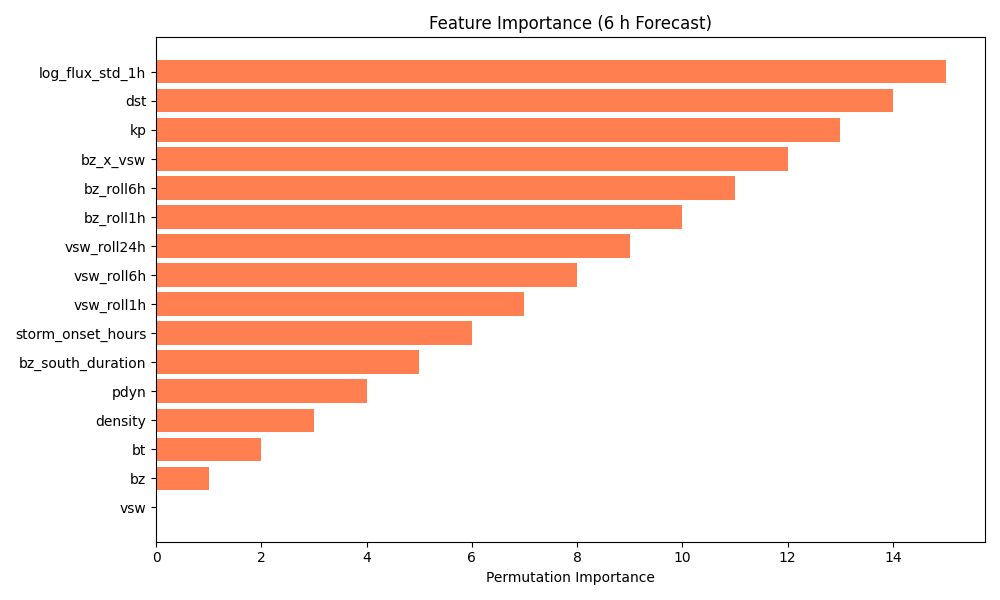
\includegraphics[width=0.92\columnwidth]{figures/fig_feature_importance.png}
\caption{Permutation importance (\(6\,\mathrm{h}\) PE drop) for STORM-BzGate.}
\label{fig:perm}
\end{figure}


\subsection{Interpretability}
\begin{figure}[t]
\centering

\includegraphics[width=0.88\columnwidth]{figures/fig6_delay_hist.png}
\caption{Learned propagation delay \(\tau\) across STORM seeds. The tight
concentration at 1.5\,h recovers the physical L1 transit time.}
\label{fig:delay}
\end{figure}

\begin{figure}[t]
\centering

\includegraphics[width=0.88\columnwidth]{figures/fig7_gate_activation.png}
\caption{\(B_z\) gate activation: storm windows (orange) show lower activation
values than quiet periods (blue), confirming physics-aware behavior.}
\label{fig:gate}
\end{figure}

The converged \(\tau\approx1.5\,\mathrm{h}\) (Fig.~\ref{fig:delay}) corresponds
to a solar wind speed of \(\approx370\,\mathrm{km\,s^{-1}}\), close to the
multi-year mean in our training data and consistent with published propagation
time estimates~\cite{forsyth2020}. We did not hard-code that value; the
optimizer found it from the forecast loss. Gate activations
(Fig.~\ref{fig:gate}) shift during storm intervals relative to quiet hours.
That shift is modest---many ``storm'' hours are already in recovery---but it
is consistent across seeds, which is what we need for a qualitative check
rather than a formal causal claim.

\subsection{GRASP Transfer}
Zero-shot transfer fails hard (Table~\ref{tab:grasp}). The GOES-trained
Transformer falls to PE\(_{6h}=-2.16\); the main practical causes are the
15-versus-16 feature mismatch after alignment and shifts in the solar-wind
marginals between the two longitudes. STORM-BzGate zero-shot is closer to
zero than the Transformer, but still not useful as an operational product
without adaptation.

Frozen-encoder fine-tuning---updating only the input projection and the output
heads, about \(73\)K parameters---recovers PE\(_{6h}=0.564\) and, more
importantly for operations, the best storm-time PE (0.529) and high-flux PE
(0.689) among the strategies we tried. Full fine-tuning and training from
scratch reach higher PE\(_\mathrm{all}\) but give back storm and high-flux
skill, which is the opposite of what a radiation-hazard user wants. With half
of the GRASP training data, frozen transfer already approaches the full
frozen curve. That matters for a newly commissioned Indian GEO payload that
will not have years of local labels on day one. We still treat the absolute
GRASP PE with caution: only 118 storm hours sit in the test window.

\begin{table}[t]
\centering
\caption{GRASP transfer (storm: 118/1781 windows). Bold: best.}
\label{tab:grasp}
\setlength{\tabcolsep}{3.2pt}
\begin{tabular}{lcccc}
\toprule
Experiment & PE\(_{45\mathrm{m}}\) & PE\(_{6\mathrm{h}}\) & PE\(_{\mathrm{st}}\) & PE\(_{\mathrm{hi}}\) \\
\midrule
Zero-shot TF & \(-32.22\) & \(-2.16\) & \(-7.64\) & \(-16.65\) \\
Zero-shot BzGate & \(\approx0\) & \(\approx0\) & \(\approx0\) & 0.02 \\
Frozen TL & 0.18 & 0.56 & \textbf{0.53} & \textbf{0.69} \\
Full TL & 0.25 & 0.68 & 0.18 & 0.60 \\
Scratch & 0.25 & 0.69 & 0.18 & 0.47 \\
Few-shot 50\% & 0.23 & 0.64 & 0.53 & 0.66 \\
Few-shot 100\% & \textbf{0.29} & \textbf{0.72} & 0.33 & 0.68 \\
\bottomrule
\end{tabular}
\end{table}

\begin{figure}[t]
\centering

\includegraphics[width=\columnwidth]{figures/fig8_grasp_domain_gap.png}
\caption{GRASP domain transfer at 6\,h. Frozen TL dramatically recovers over
zero-shot, with best storm and high-flux performance.}
\label{fig:grasp}
\end{figure}

%% ====================================================================
\section{Limitations and Conclusion}
%% ====================================================================
Several limits should stay in view. Only three random seeds are available for
the main STORM comparisons, so formal significance tests remain exploratory.
GRASP spans only about 14 months in a quiet declining phase of Solar Cycle 24,
and storm PE there is based on 118 test hours, so the uncertainty is larger than
on the GOES test set. Aggregate 6\,h PE moves little under ablations; the physics
terms show up mainly in storm PE. Monte Carlo dropout coverage on a sample
checkpoint was well below a nominal 90\% band, so we do not claim calibrated
uncertainty. Published PE numbers in the literature use mixed cadences, energy
channels, and persistence definitions, so we do not claim a cross-paper ranking
from raw PE alone~\cite{morley2018,camporeale2019}. The backbone is a temporal
Transformer; it does not explicitly model variate-axis interactions the way an
iTransformer would, which may matter during fast CME-driven transitions.

Within those bounds, STORM-PhysNet is a reproducible multi-horizon baseline on
GOES and a concrete transfer recipe for GRASP. The \(B_z\)-gated model improves
storm-time PE by a few points over a matched Transformer and, at 45\,min,
avoids the seed-to-seed collapses we saw in the baseline. Removing the delay or
the physics loss each costs storm skill. Frozen-encoder adaptation recovers
usable Indian-longitude forecasts with a small trainable subset after GOES
pretraining. The learned delay near \(1.5\,\mathrm{h}\) lines up with typical
L1 transit times, which is a useful sanity check even though it is not a formal
physics proof. Future work can extend the GRASP window across a fuller solar
cycle and test whether EUV or multi-orbit inputs tighten the short-horizon
tail further.

\section*{Data Availability}
GOES-15 EPEAD and OMNI datasets are available from public archives. GRASP data is used under the specific terms of the problem setting.

\section*{Acknowledgments}
The authors thank the GOES, OMNI, and GRASP data providers.

\begin{thebibliography}{99}
\bibitem{baker1990}
D.~N. Baker et al., ``Linear prediction filter analysis of relativistic
electron properties at 6.6 \(R_E\),'' \emph{J. Geophys. Res.}, vol.~95,
pp.~15133--15140, 1990.

\bibitem{perry2010}
K.~A. Perry et al., ``Comparing geosynchronous relativistic electron
prediction models,'' \emph{Space Weather}, vol.~8, S12003, 2010.

\bibitem{ling2010}
A.~G. Ling et al., ``Identifying solar wind drivers of radiation belt
responses,'' \emph{Space Weather}, vol.~8, no.~10, 2010.

\bibitem{wei2018}
L.~Wei et al., ``Quantitative prediction of high-energy electron integral flux
at GEO based on deep learning,'' \emph{Space Weather}, vol.~16,
pp.~903--916, 2018.

\bibitem{camporeale2019}
E.~Camporeale, ``The challenge of machine learning in space weather,''
\emph{Space Weather}, vol.~17, pp.~1166--1207, 2019.

\bibitem{morley2018}
S.~K. Morley et al., ``Evaluating the performance of radiation belt models,''
\emph{Space Weather}, vol.~16, pp.~1521--1548, 2018.

\bibitem{baker2018space}
D.~N. Baker et al., ``Space weather effects in the Earth's radiation belts,''
\emph{Space Sci.\ Rev.}, vol.~214, p.~17, 2018.

\bibitem{horne2005wave}
R.~B. Horne et al., ``Wave acceleration of electrons in the Van Allen
radiation belts,'' \emph{Nature}, vol.~437, pp.~227--230, 2005.

\bibitem{son2022}
J.~Son et al., ``72-hour forecasting of hourly relativistic electron fluxes at
GEO by deep learning,'' \emph{Space Weather}, vol.~20, e2021SW002985, 2022.

\bibitem{sun2024swsc}
X.~Sun et al., ``\(\ge2\) MeV electron fluxes in GEO at different prediction
time scales: LSTM and transformer,'' \emph{J. Space Weather Space Clim.},
vol.~14, p.~20, 2024.

\bibitem{tan2024tpa}
W.~Tan et al., ``TPA-LSTM and Transformer for GEO radiation belt electron
fluxes,'' \emph{Space Weather}, vol.~22, e2023SW003714, 2024.

\bibitem{sun2025fsl}
X.~Sun et al., ``Enhancing \(\ge2\) MeV electron fluence predictions in GEO
through deep learning strategies,'' \emph{Space Weather}, vol.~23,
e2024SW003975, 2025.

\bibitem{sinha2021premeve}
S.~Sinha et al., ``PreMevE update,'' \emph{Space Weather}, vol.~19,
e2020SW002671, 2021.

\bibitem{kieokaew2026timesfm}
R.~Kieokaew et al., ``Forecasting MeV electron flux using ML and a timeseries
foundation model,'' arXiv:2605.15752, 2026.

\bibitem{forsyth2020}
C.~Forsyth et al., ``Forecasting GOES 15 \(>2\) MeV electron fluxes,''
\emph{Space Weather}, vol.~18, e2020SW002527, 2020.

\bibitem{zhang2022emd}
H.~Zhang et al., ``EMD-LSTM for relativistic electrons at GEO,''
\emph{Space Weather}, vol.~20, e2022SW003100, 2022.

\bibitem{simms2020}
L.~E. Simms et al., ``Classifier neural network models predict relativistic
electron events at geosynchronous orbit,'' \emph{J. Geophys. Res.\ Space
Physics}, vol.~125, e2019JA027323, 2020.

\bibitem{tang2022}
R.~Tang et al., ``Short-time prediction of energetic electron flux based on
stacking ensemble learning,'' \emph{Space Weather}, vol.~20,
e2021SW002928, 2022.

\bibitem{botek2023}
E.~Botek et al., ``Prediction of radiation belt electron fluxes at LEO using
neural networks,'' \emph{Space Weather}, vol.~21, e2022SW003345, 2023.

\bibitem{turner2012}
D.~L. Turner et al., ``Explaining sudden losses of outer radiation belt
electrons during geomagnetic storms,'' \emph{Nature Phys.}, vol.~8,
pp.~208--212, 2012.

\bibitem{vaswani2017}
A.~Vaswani et al., ``Attention is all you need,'' \emph{NeurIPS}, 2017,
pp.~5998--6008.

\bibitem{liu2024itrans}
Y.~Liu et al., ``iTransformer: Inverted Transformers are effective for time
series forecasting,'' in \emph{Proc.\ ICLR 2024} (Spotlight), 2024.
arXiv:2310.06625.

\end{thebibliography}
\balance
\end{document}
